\documentclass{article}
\usepackage{multirow}
\usepackage{hyperref}
\usepackage{graphicx}
\usepackage{xcolor}
\usepackage{float}

\title{Root Digger: a root placement program for phylogenetic trees}
\author{Ben Bettisworth, Alexandros Stamatakis}
\date{\today}

\newcommand{\RootDigger}{RootDigger}
\newcommand{\RootDiggertt}{\texttt{RootDigger}}
\newcommand{\BenComment}[1]{{\bf \color{blue} ({#1})}}
\newcommand{\AlexisComment}[1]{{\bf \color{green} ({#1})}}

\begin{document}
\begin{abstract}
  In phylogenetic analysis, it is common to infer trees which are unrooted.
  This is to say, it is unknown which node is the most recent common ancestor of
  all the taxa present in the phylogenetic tree.
  This information is often desirable, as it provides a direction to the edges in
  the tree.
  There exist several methods to recover a root, including midpoint rooting and
  using a special taxon as a so called outgroup.
  Additionally, a non-reversable Markov model can be used to compute the
  likelihood of a root.
  In this paper, we present software which uses a provided non-reversable model
  to compute the most likely root location.
\end{abstract}

\maketitle

% Main Points:
% - Rerunning analysis with outgroups is expensive, and can introduce errors
% - Midpoint rooting is a joke
% - This is fast and accurate.

\section{Introduction}

% Outline:
% - What is rooting
% - Why do we need it
% - Existing methods
% - What this method is
% - Why should we use this method

When inferring phylogenetic trees, many phyogenetic inference tools
\cite{stamatakis_raxml_2014} \cite{nguyen_iq-tree:_2015} will infer an unrooted
tree.
This is due to a common (and default) assumption: reversibility of the
character substitution process \cite{felsenstein_evolutionary_1981}.
This assumption yields the problem of inferring a phylogenetic tree much more
computationally tractable, however by making this assumption the ability to
distinguish a root is lost.
A rooted phylogenetic tree is desirable, though, as it can resolve long
standing disputes regarding the placement of large clades on the tree of life
\cite{dunn_animal_2014} for example.

There are several methods to recover the root on an existing phylogenetic tree,
which generally fall into one of three categories: methods which use additional
topological information not present in the molecular data; methods which
utilize some variation of the molecular clock hypothesis; and methods which use
a non-reversible model.

Methods that use additional topological information take advantage of prior
knowledge about the world, which isn't present in the data that is used to
infer a tree.
In particular, knowledge about species which are distantly related can be used
to add a so-called outgroup to phylogenetic analysis.
This outgroup can then be used to place the root on the tree, as the most
recent common ancestor of the ingroup and the outgroup must be the root of the
tree.

There are challenges to adding an outgroup to an analysis.
Gatsey et.al.
\cite{gatesy_how_2007} showed how adding a single taxon to an analysis can
substantially change the resulting tree topology, even for the taxa which were
already present in the analysis before (i.e. the ingroup).
Holland \cite{holland_outgroup_2003} investigates this phenomenon in
simulations, and finds that outgroups affecting the topology of ingroups are
common.

Alternatively, molecular clock analysis can be used to place a root without
prior topological knowledge \cite{yang_computational_2006}.
The molecular clock hypothesis states that base substitution "ticks" at
stochastically constant rate.
Using this assumption, or some variant, a likely location can be inferred for
the root on an existing phylogenetic tree.
A simple version of this analysis is midpoint rooting, which uses a constant
molecular clock assumption.

Molecular clock analysis exhibit their own difficulties.
In particular, the clock does not "tick" at a constant rate over the tree as
shown in \cite{li_molecular_1987} and \cite{steiper_primate_2006}.
Relaxed clock models exist which can alleviate this problem, but are not always
successful as shown in \cite{battistuzzi_performance_2010}.

The final method that can place a root on a tree is to perform the phylogenetic
analysis using a non-reversible model.
By using a non-reversible model, we can place a direction of time on the
branches of a tree \cite{yap_rooting_2005}.
Several software packages are able to infer a phylogenetic tree under an
non-reversible model, thereby inferring a root \cite{nguyen_iq-tree:_2015}
\cite{ronquist_mrbayes_2003}.

Non-reversible models for phylogenetic trees come in many forms.
For example, accounting for duplication, transfer and loss events yields a
non-reversible model \cite{morel_generax:_2019}.
In particular, duplication events have been used to root a tree
\cite{emms_stride:_2017}.
Another method, the one primarily used for this work, is to eliminate the
reversibility assumption of standard character (e.g. nucleotide or amino acid)
substitution models.
Unfortunately, eliminating this assumption will significantly increase the
computational effort required to find a good (high likelihood) phylogenetic
tree.
This is due to the loss of the pulley principle
\cite{felsenstein_evolutionary_1981}, which allows phylogenetic inference tools
to ignore placement of the root during tree inference.
Therefore, by adopting a non-reversible model, the location of a root on a
phylogenetic tree effects the likelihood of that tree.

Since the root location affects the likelihood of the tree, then using
traditional tree inference techniques all possible rootings would need to be
evaluated for each tree in order to find the rooting with highest likelihood.
In the worst case, this increases the work {\em per tree} by a factor of
$\mathcal{O}(n)$ where $n$ is the number of taxa present in the dataset.
While there are heuristics to reduce the amount of work required
\AlexisComment{For instance?
  Citation!
}\BenComment{I know this to be true, because I have talked with Benoit and
  found some heuristics myself for this project.
  I don't really know how to cite/explain this though.
  I am really just trying to be charitable to the other tools.
}, eliminating the reversibility assumption drastically increases the effort
required to infer a tree.

As an alternative to the computationally expensive process of inferring a tree
with a root, an unrooted tree which has already been inferred under a
reversible model can be evaluated for possible root locations under a
non-reversible model.
This is faster, as it skips the expensive step of looking for good rootings
during intermediate trees.
With this method, we can find the most likely root location for a given
phylogenetic tree.
There are still challenges though, as the likelihood function for rooting a
phylogenetic tree may exhibit several local maxima
\cite{huelsenbeck_inferring_2002}, though these concerns were not found to be a
major concern in our experiements.

The input to \RootDiggertt{} then is a multi-species alignment (MSA) and a
phylogenetic tree with branch lengths given in substitutions per site.
\RootDiggertt{} then uses the tree and branch lengths to find the most likely
root location by calculating the likelihood of a root location under a
non-reversible substitution model.
The likelihood of a root along a branch is calculated by splitting the given
branch into 2 branches with branch lengths $\alpha t$ and $(1-\alpha) t$, $0
  \leq \alpha \leq 1.0$.
We then find the maximum likelihood $\alpha$, and report the likelihood for
given branch as the likelihood of the root location.
By formulating the problem this way, we can use single parameter optimization
techniques such as Brent's Method\footnotemark{}, which are computationally
more efficient compared to multi-parameter optimization routines.

\footnotetext{We could compute a derivative, but the library that we use
  computes log-likelihoods, and we require plain likelihoods to compute a
  second
  derivative.
  The effort to rewrite the functions that would compute this derivative was
  deemed to be too much relative to the savings.
  In principle, the computation could be done.
}

A limitation of methods like Brent's is they will fail to find {\it all} the
extrema of a function if there are multiple extrema.
To compensate, we need to search for bracketing windows that can be used to
safely find extrema.
Unfortunately, we are not aware of a general method for finding such bracketing
windows, so a recursive method is employed, were the search range is reduced in
half and searched for appropriate\footnotemark{} windows.

\footnotetext{Appropriate here means that the sign of the function in question
  has opposite signs at the endpoints of the window.}

\RootDiggertt{} offers a fast and a slow method, which are placement and
exhaustive, respectively.
Search mode simply finds the most likely root quickly.
Exhaustive mode evaluates the likelihood of the root for every branch of a
given tree, and reports the likelihood weight ratio
\cite{strimmer_inferring_2002} of a root on that branch for every branch on the
tree.
In addition to the two search methods, there is an optional early stop mode,
which can be combined with either search method.
In this early stop mode, the search will conclude if the root placement is
nearly the same twice in a row.
While this mode does improve search times substantially, the likelihood of the
root placement will not be fully optimized.
In practice, this does substantially effect the final root placement, but it
does render comparison of likelihood results difficult \BenComment{Impossible?
}.

\section{Methods}

%\AlexisComment{We need to better it... this, just give an overview then go inot
%  the details, despite the uninformative mode print, then the commitee}

As mentioned in the previous section, \RootDiggertt{} has 2 modes of operation.
These modes will be discussed individually, starting with placement mode.

\begin{enumerate}
  \item Initialize numerical model parameters:
        \begin{itemize}
          \item $\Gamma$ parameter for rates to $1.0$ (if applicable),
          \item Character substitution rates to uniform random values according
                to $U(0.0001, 1.0)$,
          \item Base frequencies to uniform random values according to
                $U(0.0001, 1.0)$.
        \end{itemize}
  \item Choose starting roots by likelihood at branch midpoint.
  \item For each starting root:
        \begin{enumerate}
          \item Optimize model parameters
                \begin{itemize}
                  \item $\Gamma$ parameter for rates (if applicable),
                  \item Character substitution rates,
                  \item Base Frequencies.
                \end{itemize}
          \item Find best root location
                \begin{enumerate}
                  \item Create a list of high likelihood root locations
                        evaluated at the midpoint of every branch.
                  \item For the top roots (default 5\%), optimize the root
                        location along the branch.
                \end{enumerate}
          \item Repeat from $3.a$ until a stopping condition is met:
                \begin{itemize}
                  \item The difference between likelihoods between this
                        iteration and the previous iteration is sufficiently
                        small (below \texttt{atol}) or,
                  \item If early stopping is enabled, the new root location is
                        sufficiently close to the old root location by distance
                        along the branch (below \texttt{brtol}).
                \end{itemize}
        \end{enumerate}
  \item Report the best found root, along with its likelihood
\end{enumerate}

The process for exhaustive search is similar, with the core optimization
routines being shared with search mode.
The major difference is that all branches are attempted:

\begin{enumerate}
    \item For every branch on the tree:
    \begin{enumerate}
      \item Place root at current branch.
      \item Initialize numerical parameters:
                \begin{itemize}
                  \item $\Gamma$ parameter for rates (if applicable),
                  \item Character substitution rates,
                  \item Base Frequencies.
                \end{itemize}
          \item Optimize model parameters
                \begin{itemize}
                  \item $\Gamma$ parameter for rates (if applicable),
                  \item Character substitution rates,
                  \item Base Frequencies.
                \end{itemize}
          \item Repeat from $1.c$ until a stopping condition is met:
                \begin{itemize}
                  \item The difference between likelihoods between this
                        iteration and the previous iteration is sufficiently
                        small (below \texttt{atol}) or,
                  \item If early stopping is enabled, the new root location is
                        sufficiently close to the old root location by distance
                        along the branch (below \texttt{brtol}).
                \end{itemize}
    \end{enumerate}
  \item Report the tree with annotations for every branch:
    \begin{itemize}
      \item $\alpha$,
      \item Likelihood,
      \item and Likelihood Weight Ratio \cite{strimmer_inferring_2002}.
    \end{itemize}
\end{enumerate}

\section{The Software}

In order to implement both likelihood computations and non-reversible models,
\RootDigger{} has two major dependencies: GNU Scientific Library (GSL)
\cite{gough_gnu_2009} and the Phylogenetic Likelihood Library (LibPLL)
\cite{flouri_phylogenetic_2015}.
GSL is used to for the decomposition of a non-symmetric rate matrix, and LibPLL
is used for efficient likelihood calculation.

Usage of \RootDigger is straight-forward.
All that is required is a metric tree in newick format, and an multiple
sequence alignment (MSA) in either phylip or fasta format.
The code, documentation, experiment scripts, datasets, as well as any
modifications to existing libraries can be found at
\url{github.com/computations/root_digger}.

\section{Experiments and Results}

To validate \RootDiggertt{}, we conducted several experiments on both,
simulated, and empirical data.
Furthermore, we also used Likelihood Weight Ratios (LWR)
\cite{strimmer_inferring_2002} to asses the confidence of root placements.
Finally, we investigated how model selection affects the placement and
confidence in a particular root placement.

\subsection{Simulations}

Testing with simulated data was done to both validate the software and to
compare against IQ-TREE \cite{nguyen_iq-tree:_2015}.
To this end, we created a pipeline to

\begin{enumerate} 
  \item Generate a random tree with ETE3
        \cite{huerta-cepas_ete_2016} and random model parameters.
  \item Simulate an MSA with indelible \cite{fletcher_indelible:_2009}
  \item Run RootDigger and IQ-TREE \cite{nguyen_iq-tree:_2015} on the simulated
        MSA, given the generated random tree.
    \item Repeat from (2) for a total of 100 iterations
  \item Compute comparisons
        \begin{enumerate}
          \item Calculated rooted RF distance with ETE3
                \cite{robinson_comparison_1981}
          \item Mapped root placement onto original tree.
        \end{enumerate}
\end{enumerate}

Both IQ-TREE and \RootDiggertt{} were given the same model options for all the
runs. For all runs, the UNREST model with no rate categories was used.
Furthermore, we vary two additional parameters: MSA sites and taxa. In total, we
ran 9 simulated trials with MSA sizes of 1000, 4000, and 8000 sites as well as
tree sizes of 10, 50, and 100 taxa.
The results from these experiments are summarized in shown in figures
\ref{fig:top_error_boxplot} and \ref{fig:norm_error_boxplot}.
These experiments were timed, and the results of the timing can be found in figures
\ref{fig:iq_time_results} and \ref{fig:rd_time_results}.

\begin{figure}
  \begin{center}
    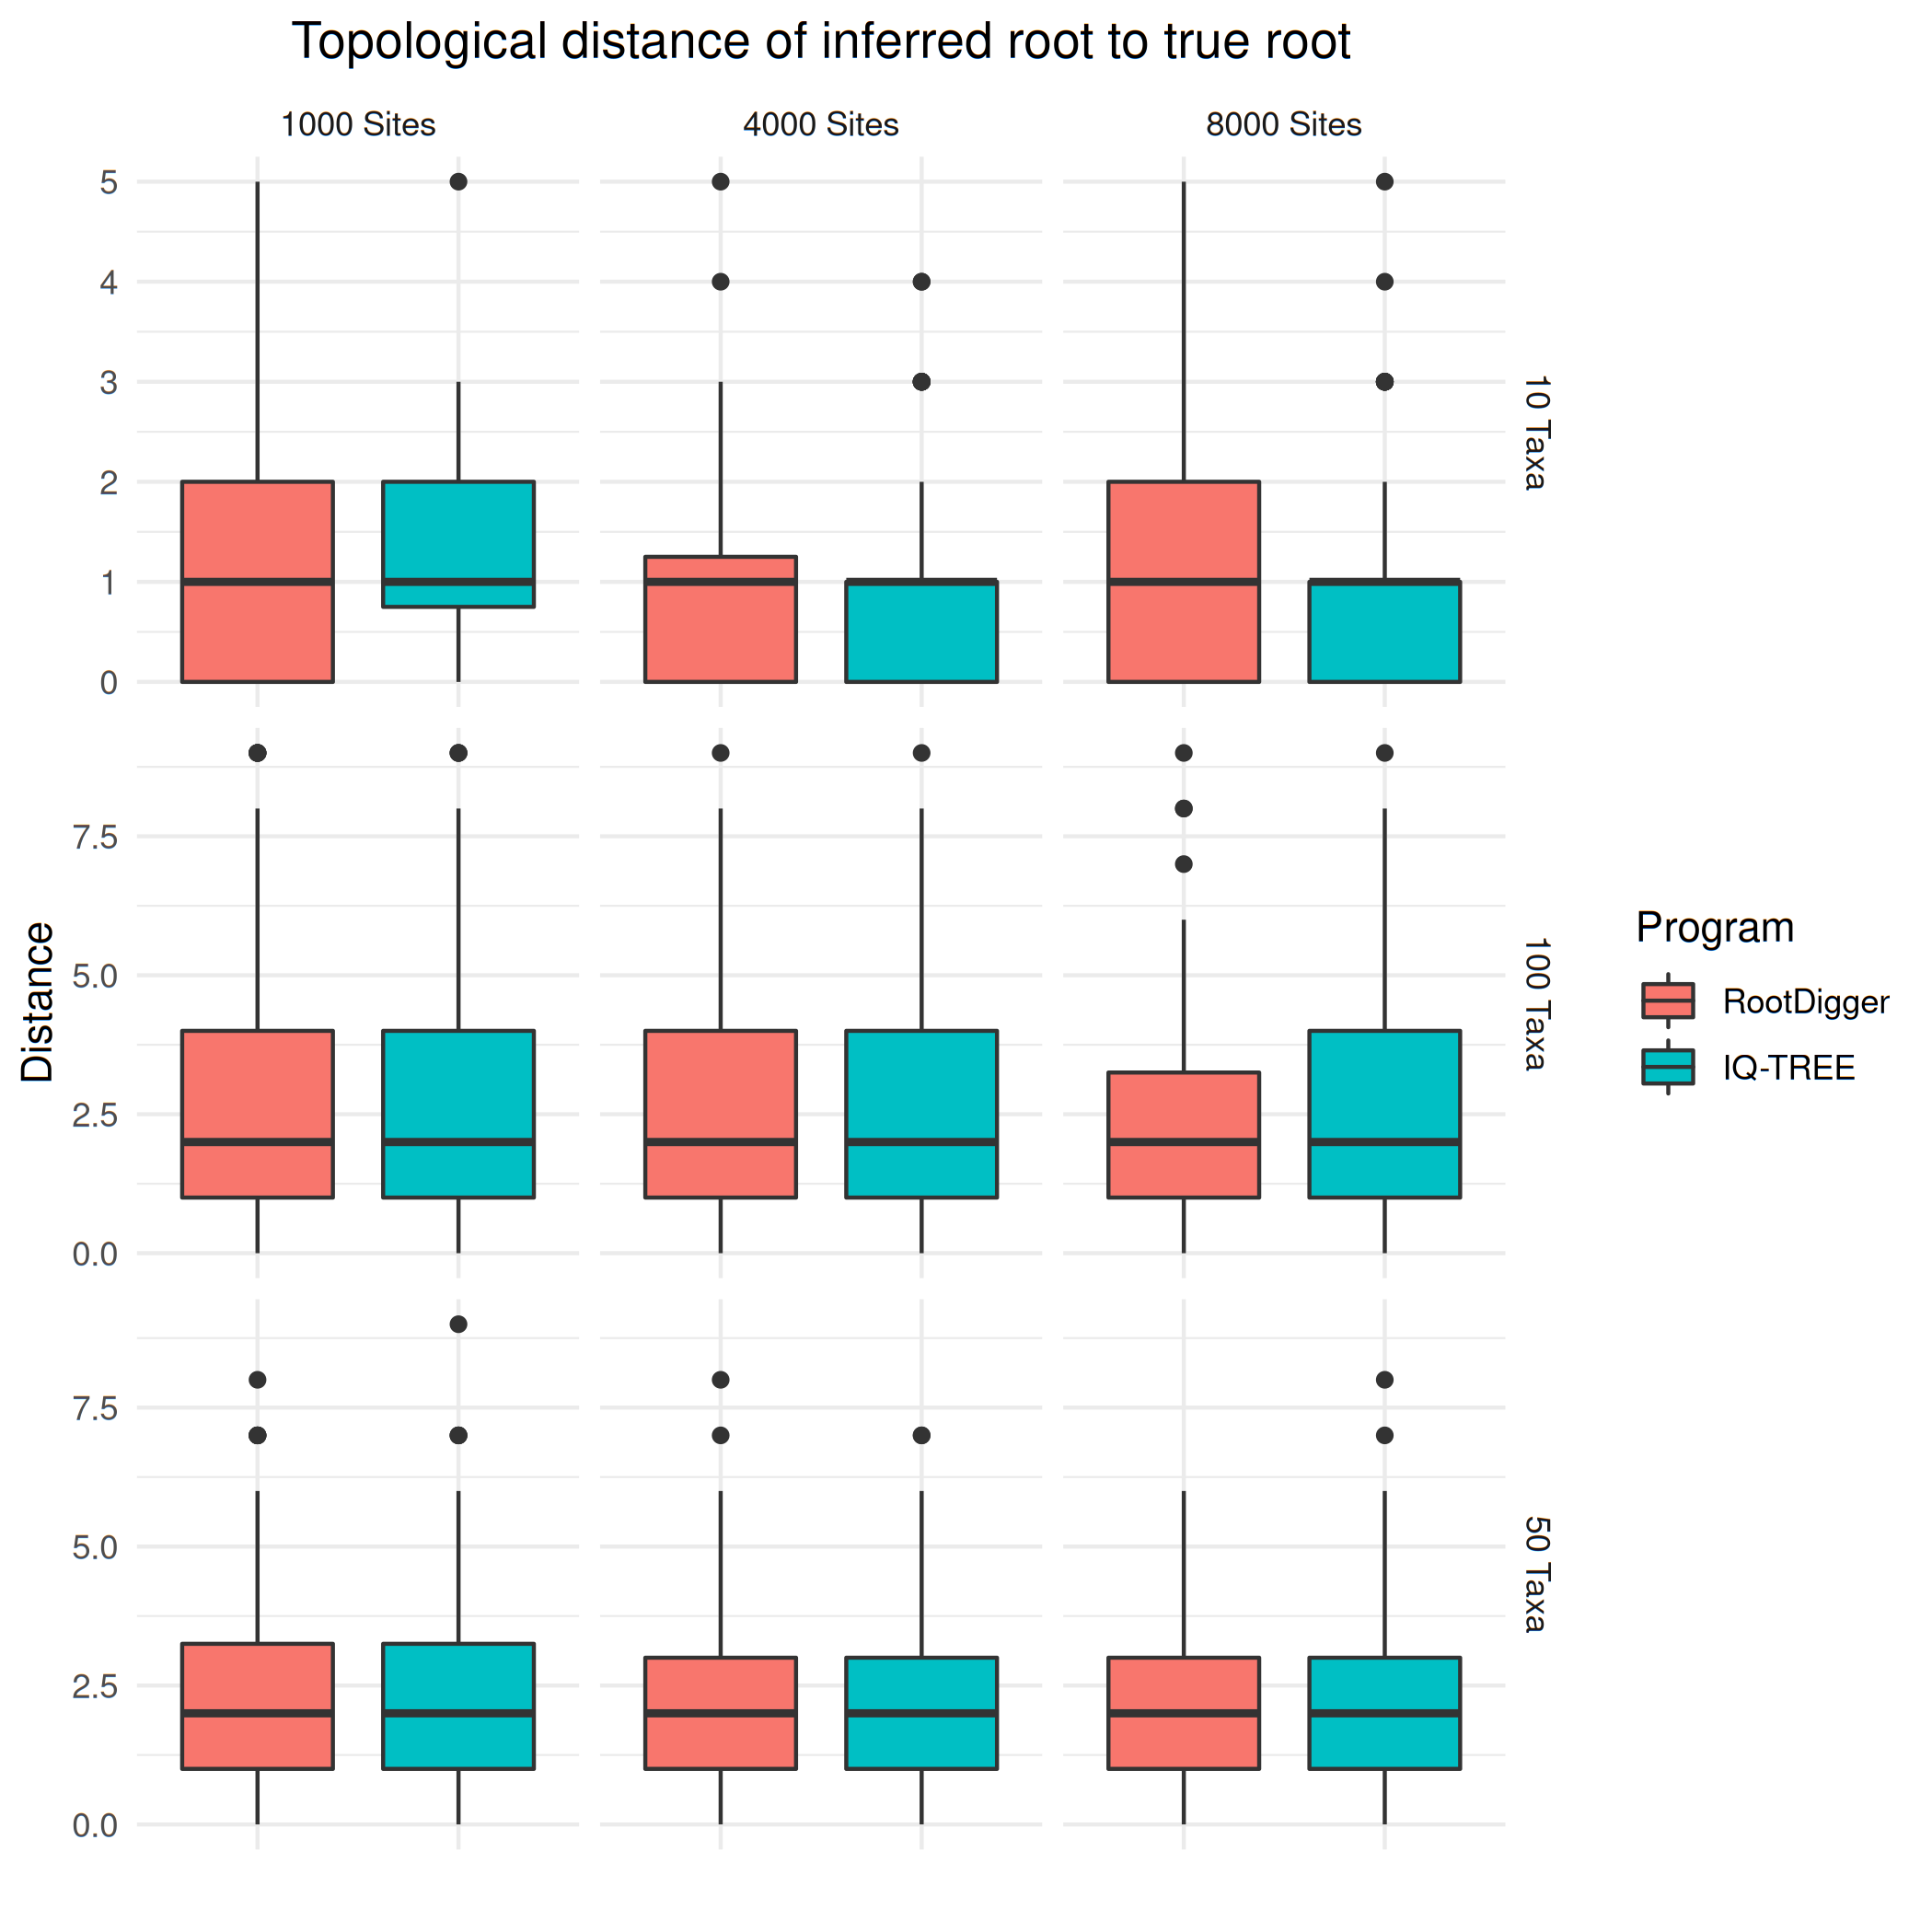
\includegraphics[width=.9\linewidth]{./figs/sim_results/melted_dist_box.png}
    \caption{Box plots of Topological error.
    \label{fig:top_error_boxplot}}
\end{center}
\end{figure}

\begin{figure}
  \begin{center}
    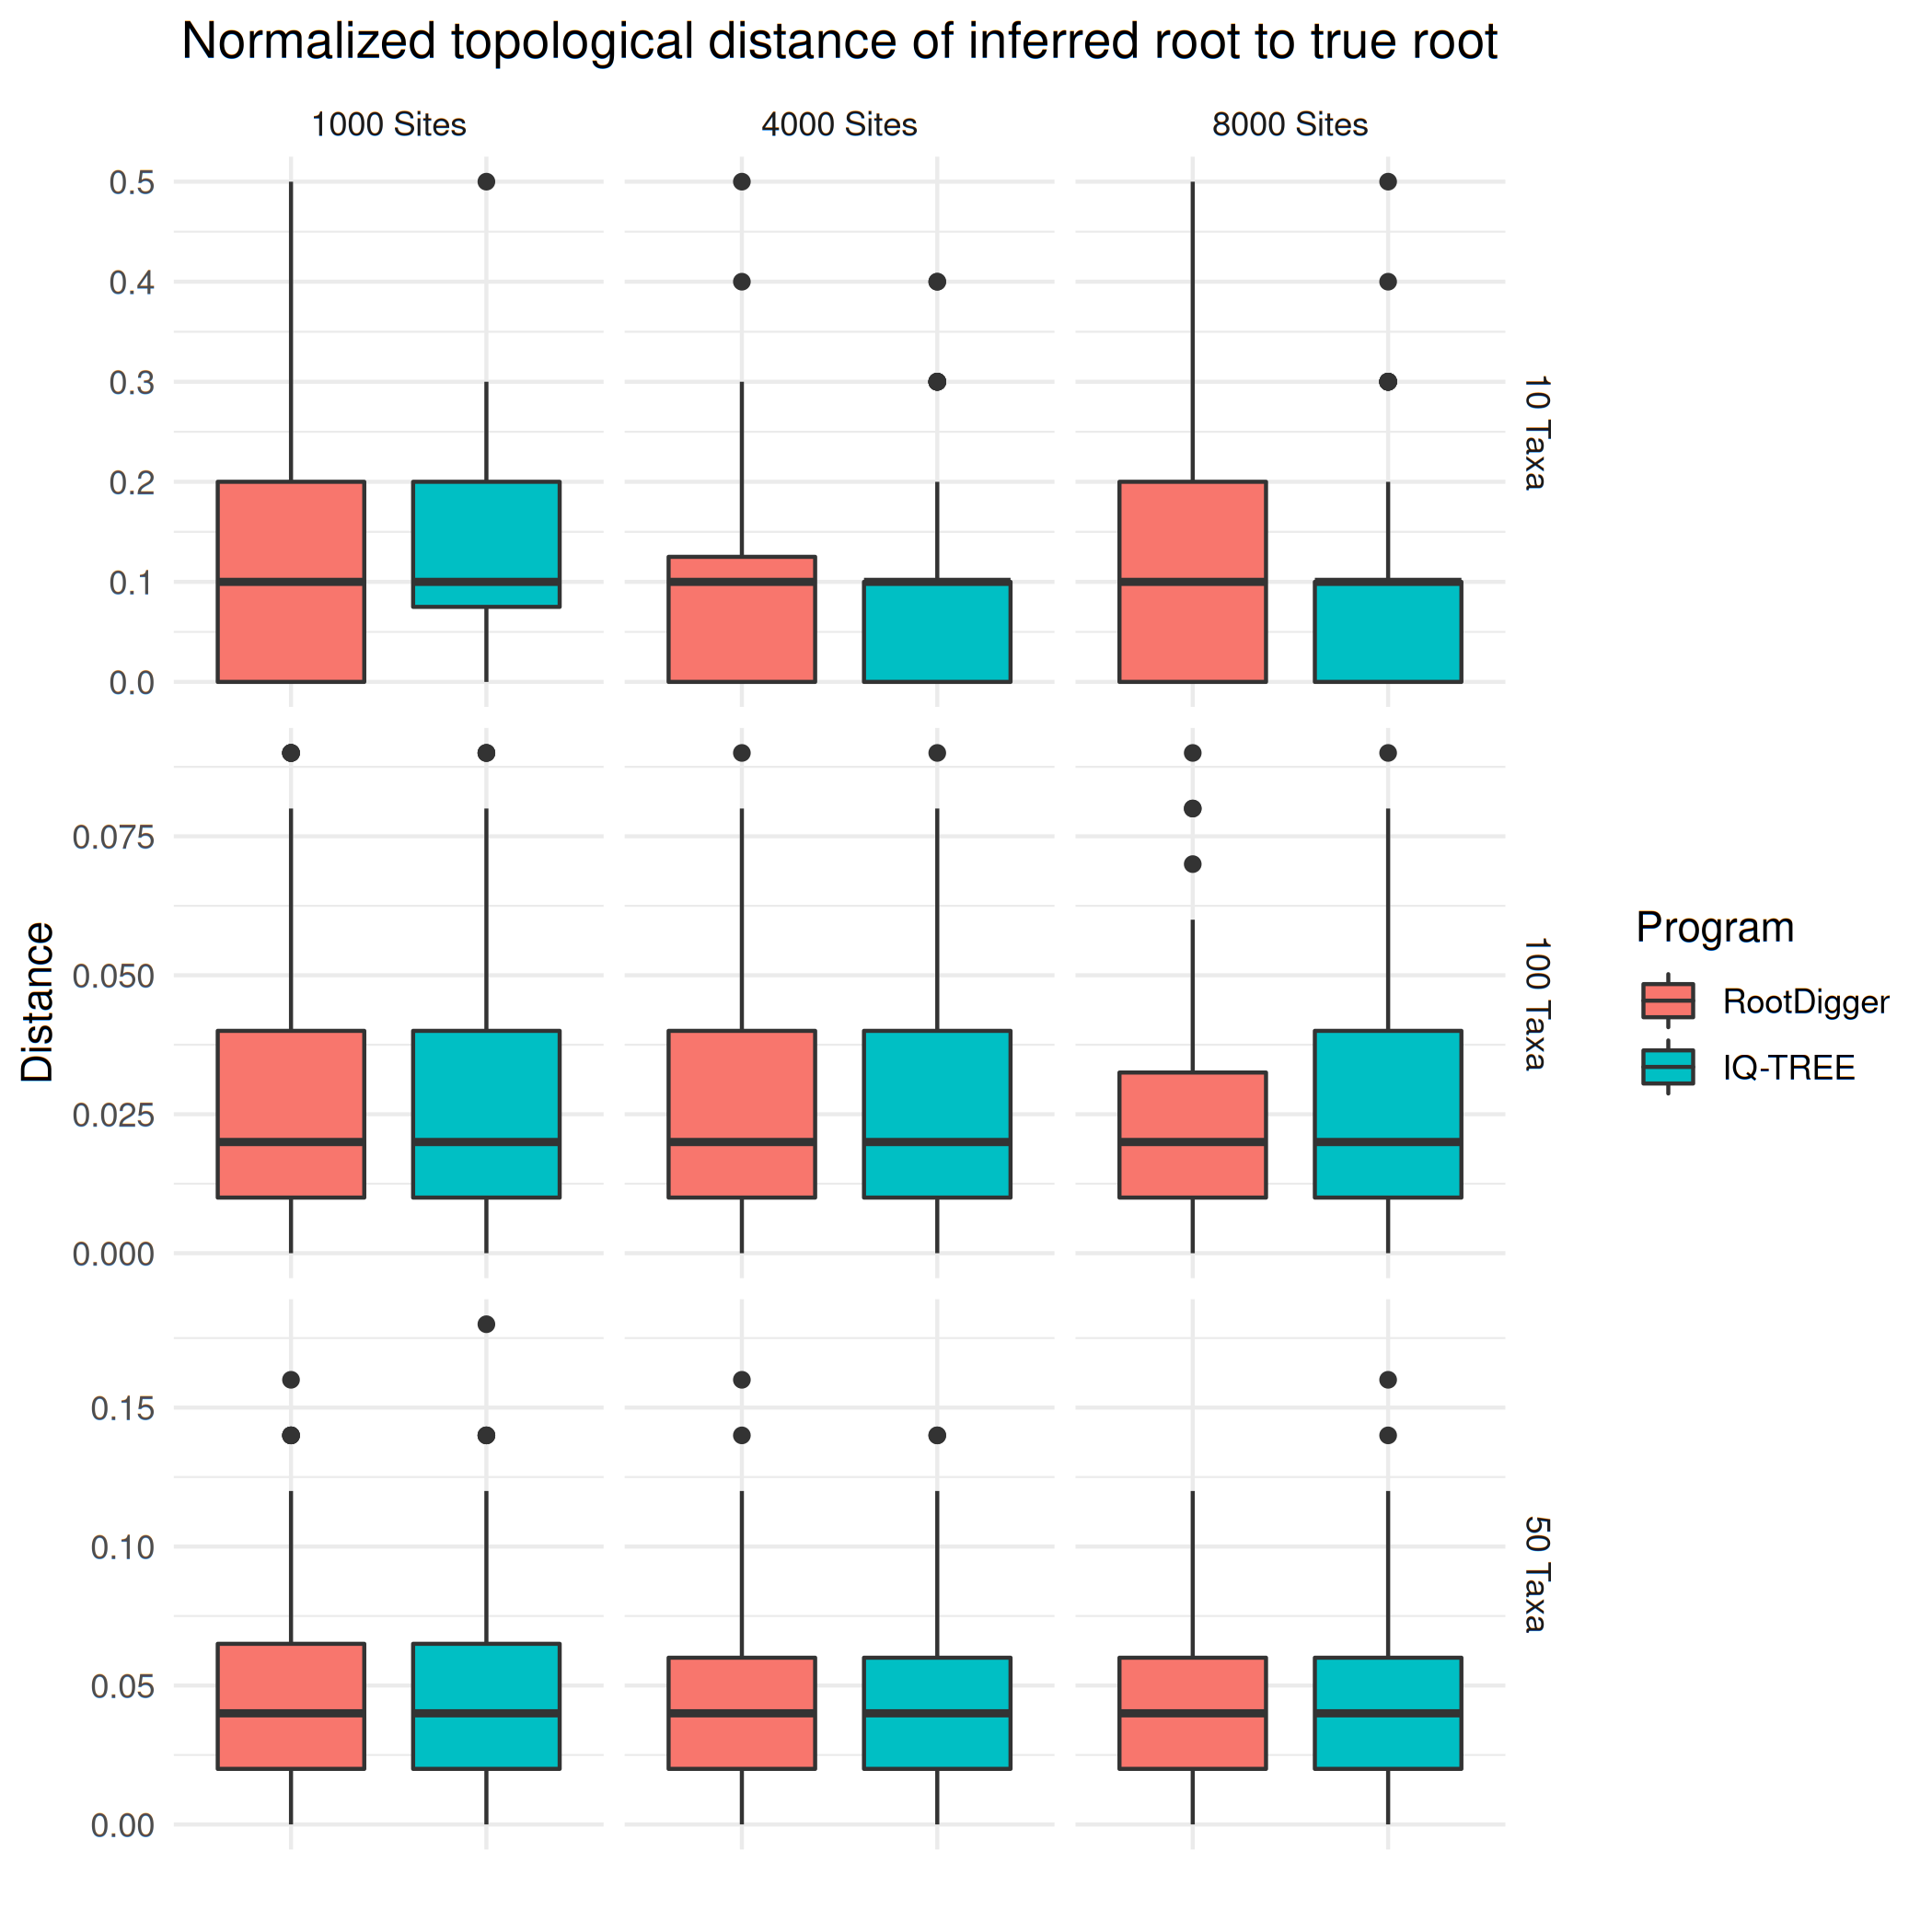
\includegraphics[width=.9\linewidth]{./figs/sim_results/melted_norm_dist_box.png}
    \caption{Box plots of normalized topological error.
    \label{fig:norm_error_boxplot}}
\end{center}
\end{figure}

\begin{figure}
  \begin{center}
    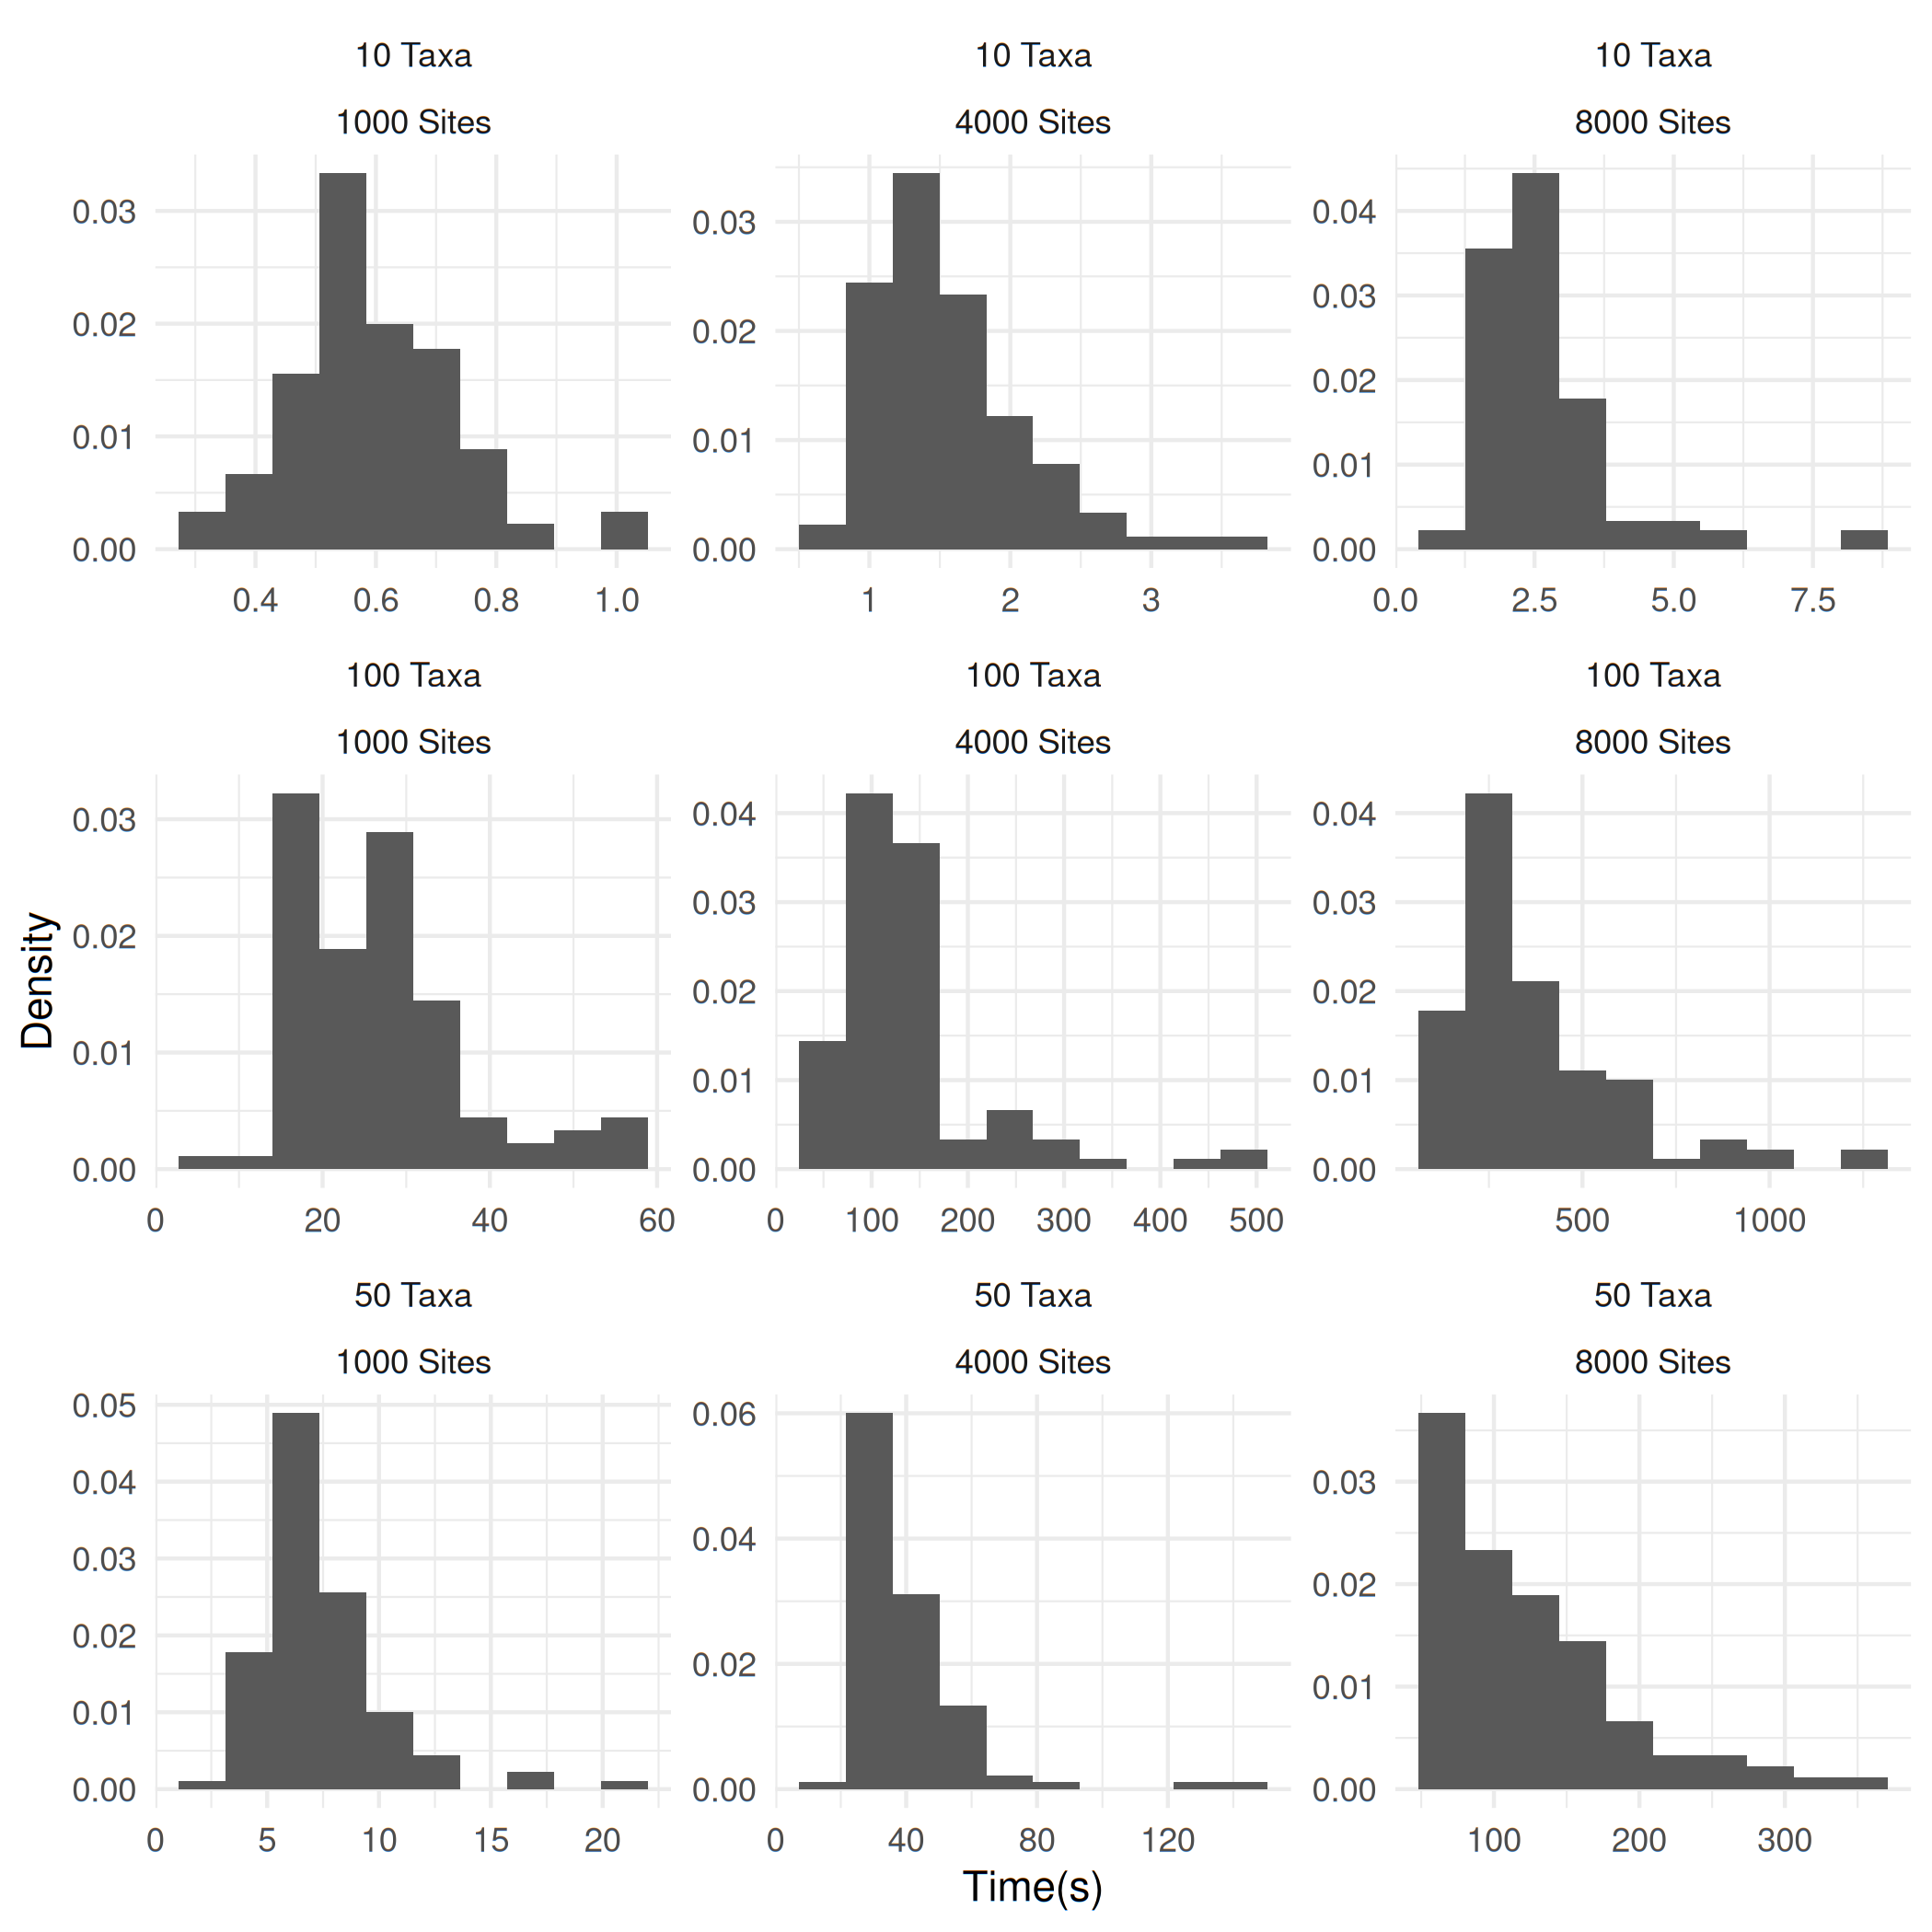
\includegraphics[width=.9\linewidth]{./figs/timing_plots/iq_time_hist.png}
  \caption{Histogram of IQ-TREE times
  \label{fig:iq_time_results}}
\end{center}
\end{figure}

\begin{figure}
  \begin{center}
    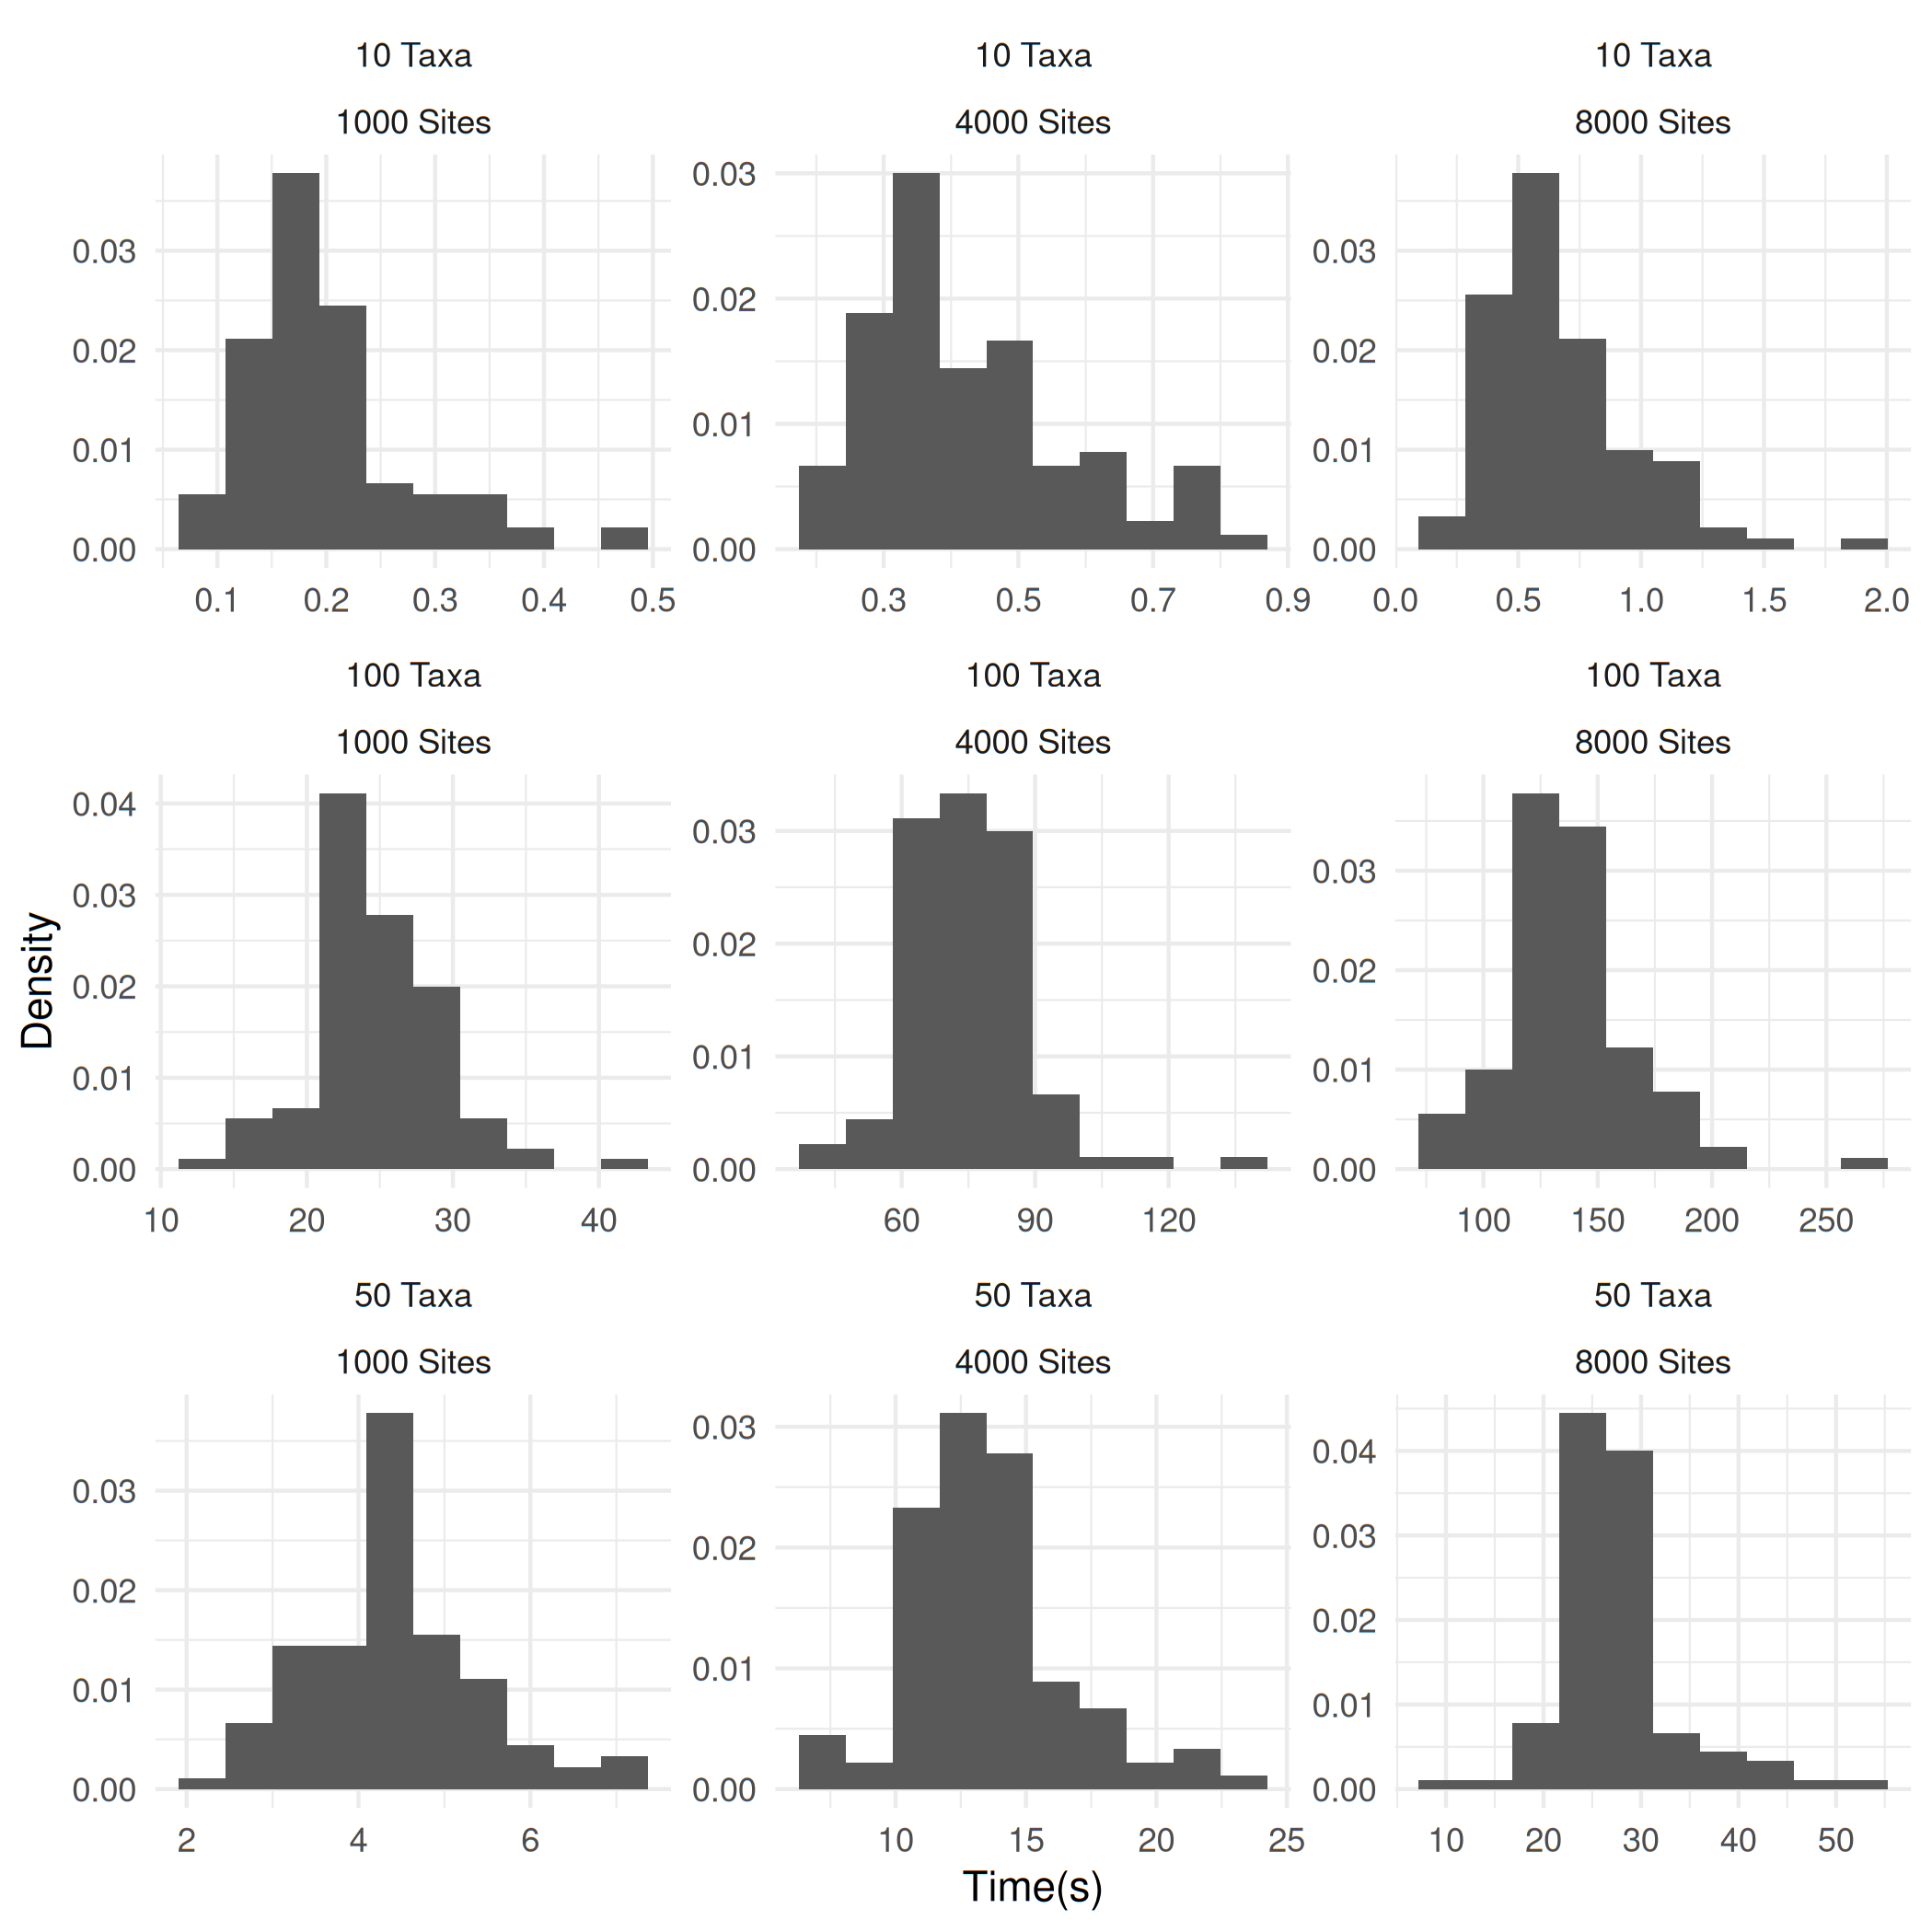
\includegraphics[width=.9\linewidth]{./figs/timing_plots/rd_time_hist.png}
    \caption{Histogram of \RootDiggertt{} times
    \label{fig:rd_time_results}}
\end{center}
\end{figure}

\begin{figure}
  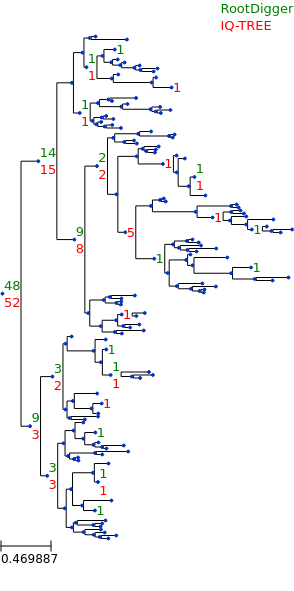
\includegraphics{figs/sim_results/100_1000.png}
  \caption{Simulation results for 100 taxa and 1000
  sites. \label{fig:sim-results-100t-1000s}}
\end{figure}

\begin{figure}
  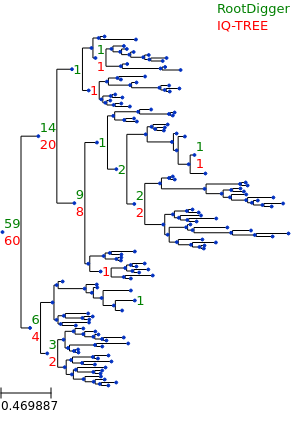
\includegraphics{figs/sim_results/100_8000.png}
  \caption{Simulation results for 100 taxa and 8000
  sites. \label{fig:sim-results-100t-8000s}}
\end{figure}

\begin{figure}
  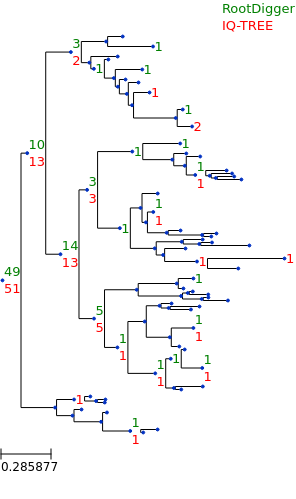
\includegraphics{figs/sim_results/50_1000.png}
  \caption{Simulation results for 50 taxa and 1000
  sites. \label{fig:sim-results-50t-1000s}}
\end{figure}

\begin{figure}
  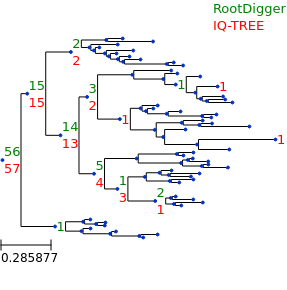
\includegraphics{figs/sim_results/50_8000.png}
  \caption{Simulation results for 100 taxa and 8000
  sites. \label{fig:sim-results-50t-8000s}}
\end{figure}

\subsection{Empirical Data}

In addition to simulated data, we conducted tests with empirical data. The
datasets used are described in \ref{table:datasets}.
The empirical datasets were chosen to have an existing, strongly supported
outgroup.
For each of the empirical datasets, we ran \RootDiggertt{} in exhaustive mode to
obtain likelihood weight ratios (LWR) for each branch.
Annotations are suppressed for branches with a small LWR (less than $0.0001$).
The trees with annotated LWR are shown in figures
\ref{fig:spiders-missing-species-no-outgroup} - \ref{fig:angio-cds12-outgroup}.
The experiments were run on datasets with the outgroup included, as well as
with the outgroup removed.

There was some preprocessing performed. Since the branch lengths in some
datasets were not specified in substitutions per site, the branch lengths were
re-optimized using RAxML-NG \cite{kozlov_raxml-ng:_2019} version
\texttt{0.9.0git}. The original model was used when it was known, otherwise the
branch lengths were optimized using GTR+G.

\begin{table}[H]
  \begin{center}
    \begin{tabular} { l c c c}
   Dataset & \#Taxa & \#Sites & Source \\
   \hline
   AngiospermsCDS12 & 35 & 864029 & \cite{ran_phylogenomics_2018}\\
   AngiospermsCDS & 35 & 1296043 & \cite{ran_phylogenomics_2018}\\
   Grasses & 245 & 4973 & \cite{christin_molecular_2014}\\
   Ficus & 200 & 5552 & \cite{cruaud_extreme_2012}\\
   SpidersMissingSpecies & 33 & 1097842 & \cite{leduc-robert_phylogeny_2018}\\
   SpidersMitocondrial & 34 & 12479 & \cite {leduc-robert_phylogeny_2018}\\
\end{tabular}
\caption{Table of emperical datasets used for validation}

    \label{table:datasets}
  \end{center}
\end{table}

%\begin{table}
%  \begin{center}
%    \begin{tabular} { l || c c  || c c  || c c || }
   Dataset & \multicolumn{2}{c ||}{Distance} & \multicolumn{2}{c ||}{Path Distance} &
   \multicolumn{2}{c ||}{Time} \\
           & RD & IQ & RD & IQ & RD & IQ \\
   \hline
   AngiospermsCDS12       & &  & & & &\\
   AngiospermsCDS         & &  & & & &\\
   Grasses                & &  & & & &\\
   Ficus                  & &  & & & &\\
   SpidersMissingSpecies  & &  & & & &\\
   SpidersMitocondrial    & &  & & & &\\
\end{tabular}
\caption{Results for empirical datasets. Distance is the distance from the
estimated root placement to the true root placement, taking into account branch
lengths. Path Distance is the topological distance from the estimated root
placement to the true root placement. RD Time and IQ time are the run times}

%    \label{table:emperical_results}
%  \end{center}
%\end{table}

\begin{figure}
  \begin{center}
    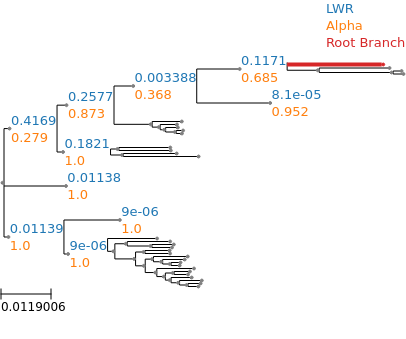
\includegraphics[width=.75\linewidth]{
    ./figs/spiders/missing_species_no_outgroup.png}
    \caption{SpidersMissingSpecies dataset analyzed without an outgroup.}
    \label{fig:spiders-missing-species-no-outgroup}
  \end{center}
\end{figure}

\begin{figure}
  \begin{center}
    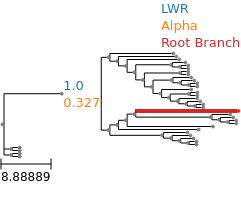
\includegraphics[width=.75\linewidth]{
    ./figs/spiders/missing_species_with_outgroup.png}
    \caption{SpidersMissingSpecies dataset analyzed with an outgroup.}
    \label{fig:spiders-missing-species-outgroup}
  \end{center}
\end{figure}

\begin{figure}
  \begin{center}
    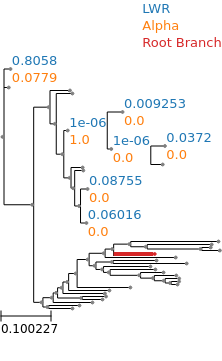
\includegraphics[width=.75\linewidth]{./figs/spiders/mito_no_outgroup.png}
    \caption{SpidersMitocondrial dataset analyzed without an outgroup.}
    \label{fig:spiders-mito-no-outgroup}
  \end{center}
\end{figure}

\begin{figure}
  \begin{center}
    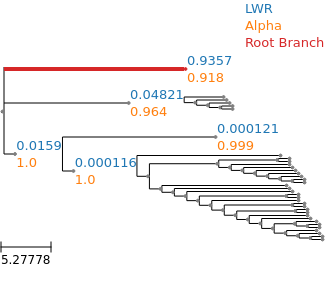
\includegraphics[width=.75\linewidth]{./figs/spiders/mito_with_outgroup.png}
    \caption{SpidersMitocondrial dataset analyzed with an outgroup.}
    \label{fig:spiders-mito-outgroup}
  \end{center}
\end{figure}

%\begin{figure}[H]
%  \begin{center}
%    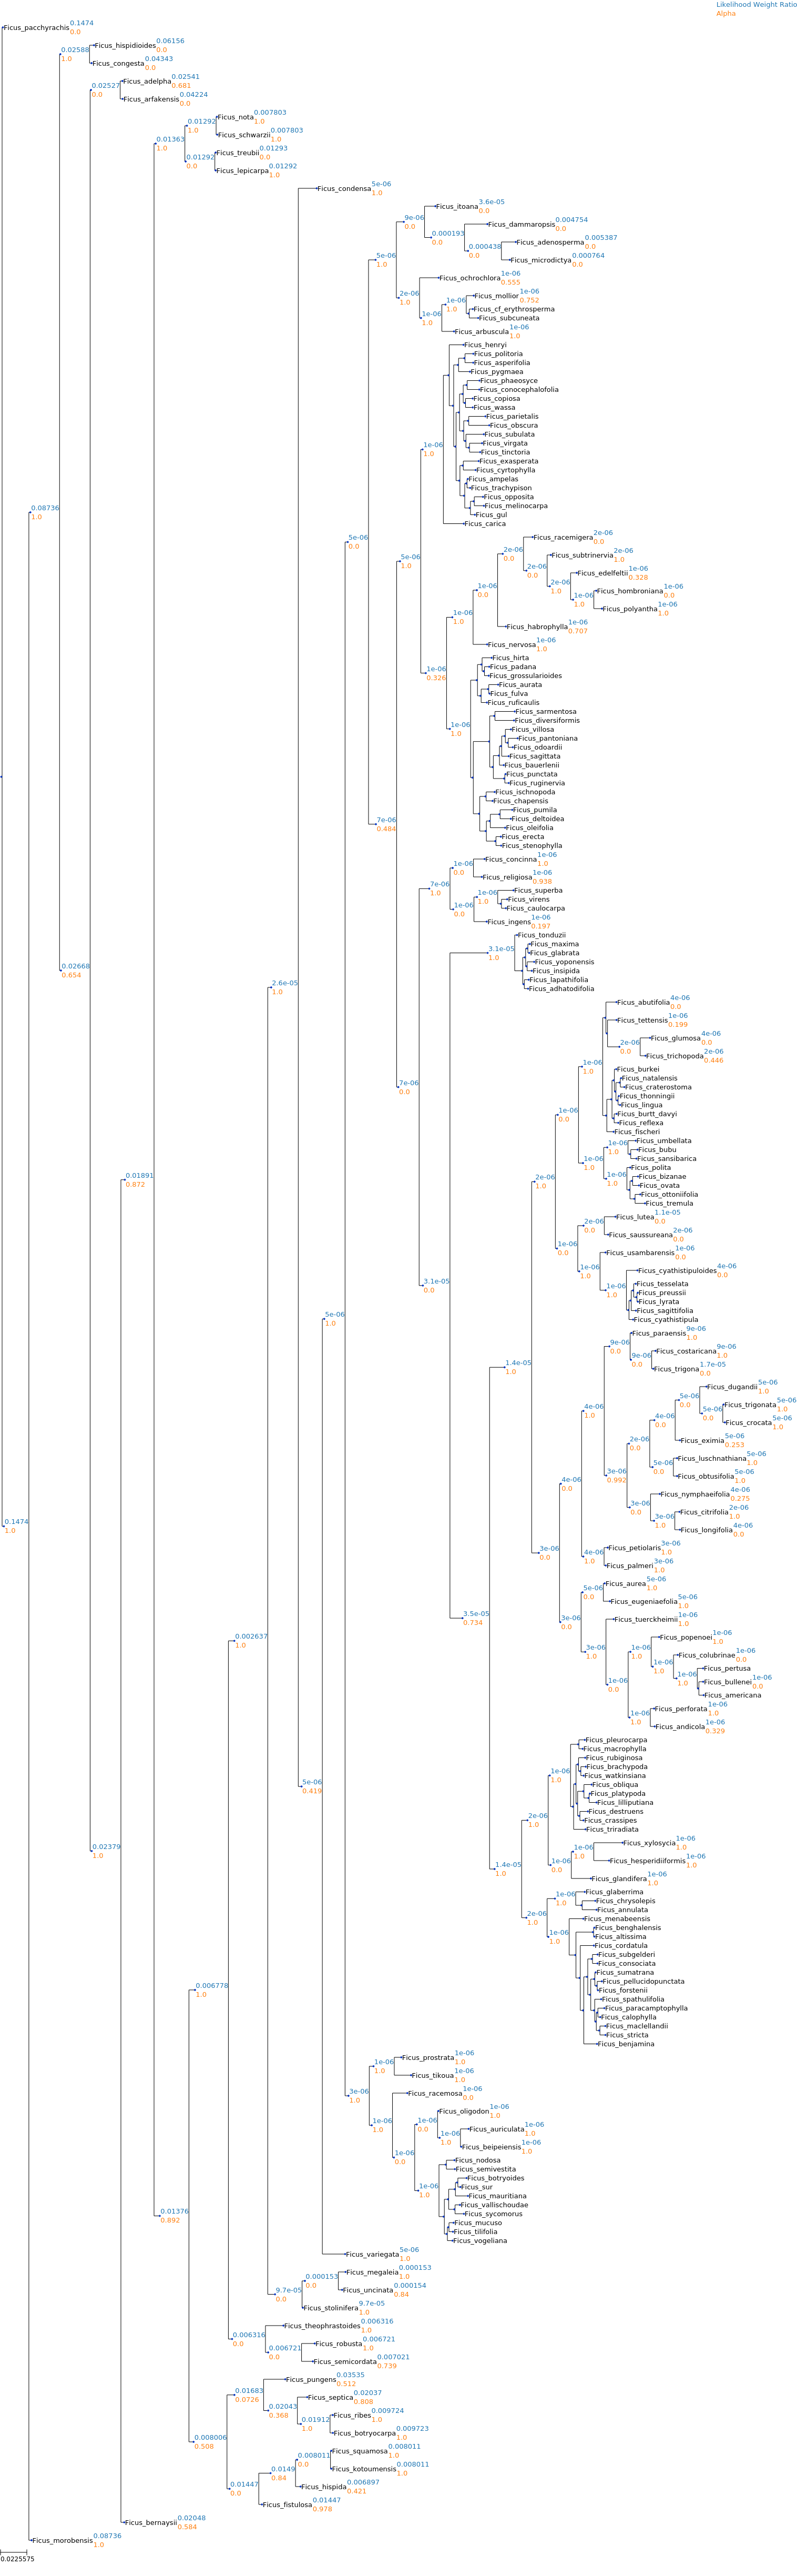
\includegraphics[width=.75\linewidth]{figs/ficus/ficus_no_outgroup_lwr.png}
%    \caption{Ficus dataset analyzed without an outgroup.}
%    \label{fig:ficus-no-outgroup}
%  \end{center}
%\end{figure}
%
%\begin{figure}[H]
%  \begin{center}
%    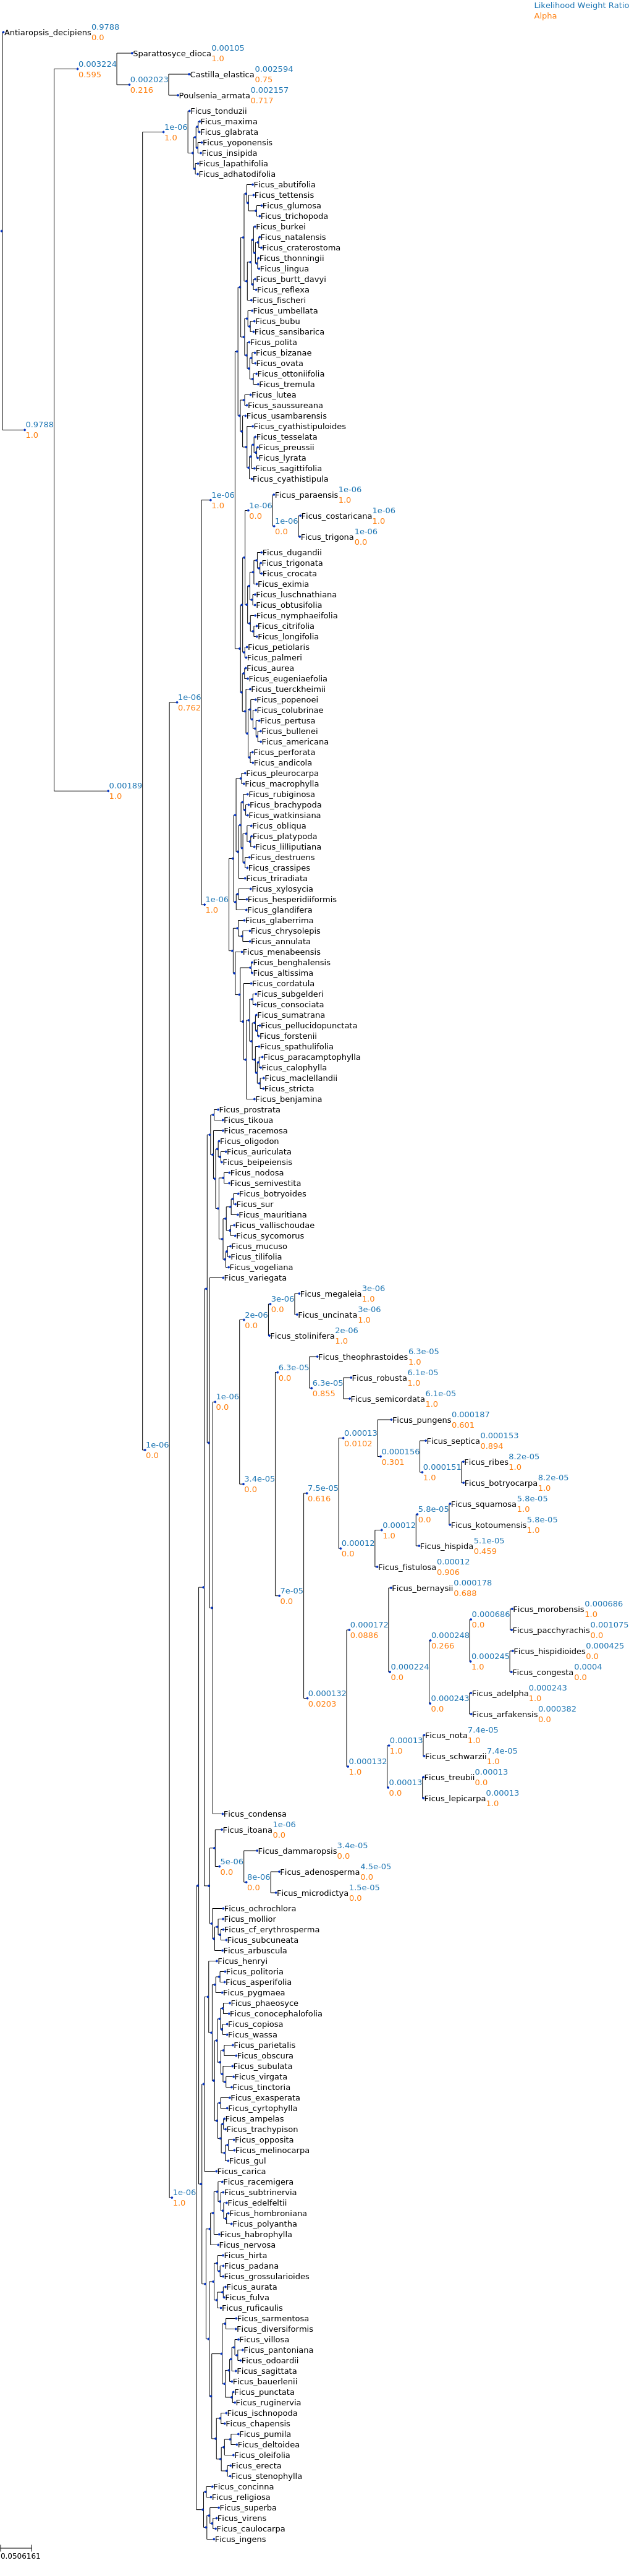
\includegraphics[width=.75\linewidth]{figs/ficus/ficus_outgroup_lwr.png}
%    \caption{Ficus dataset analyzed with an outgroup.}
%    \label{fig:ficus-outgroup}
%  \end{center}
%\end{figure}

\begin{figure}
  \begin{center}
    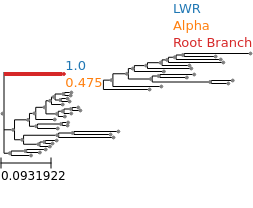
\includegraphics[width=.5\linewidth]{figs/angio/cds12_no_outgroup.png}
    \caption{AngiospermsCDS12 dataset analyzed without an outgroup.}
    \label{fig:angio-cds12-no-outgroup}
  \end{center}
\end{figure}

\begin{figure}
  \begin{center}
    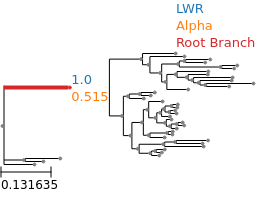
\includegraphics[width=.5\linewidth]{./figs/angio/cds12_with_outgroup.png}
    \caption{AngiospermsCDS12 dataset analyzed with an outgroup.}
    \label{fig:angio-cds12-outgroup}
  \end{center}
\end{figure}

\subsection{Effect of model selection on results}

We also investigated the effect of model selection on the results.
We did this by running \RootDiggertt{} in exhaustive mode with a varying number
of $\Gamma$ rate categories for the SpidersMitocondrial dataset.
The result of this analysis can be seen in figures~\ref{fig:spiders1rate} and
\ref{fig:spiders2rate}.
Of particular note is that increasing the number of rate categories not only
moves the root to an erroneous location, it also increases the confidence
significantly.

\begin{figure}[H]
  \begin{center}
    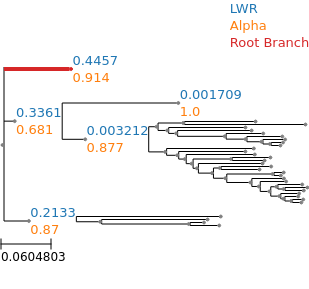
\includegraphics[width=.75\linewidth]{figs/spiders/1rate.png}
    \caption{SpidersMitocondrial dataset analyzed with 1 rate category.}
    \label{fig:spiders1rate}
  \end{center}
\end{figure}

\begin{figure}
  \begin{center}
    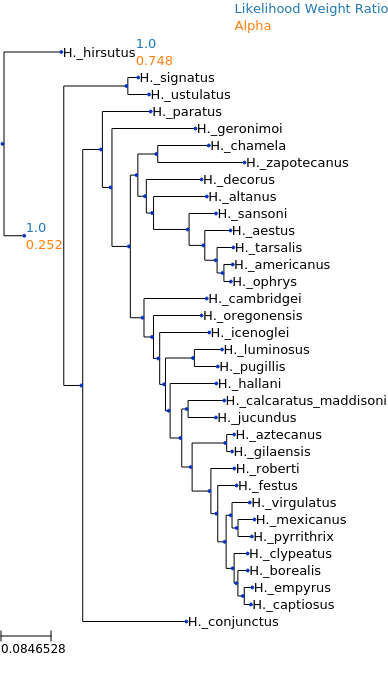
\includegraphics[width=.75\linewidth]{figs/spiders/2rate.png}
    \caption{SpidersMitocondrial dataset analyzed with 2 rate categories.}
    \label{fig:spiders2rate}
  \end{center}
\end{figure}

\subsection{Effect of early stopping on result}

Finally, we investigated the effect of the early stopping criterion on the
final LWR results. To do this, we ran \RootDiggertt{} in exhaustive mode on all
empirical datasets with early stopping enabled and disabled, resulting in paired
runs which could be compared. For most runs, the results with and without
early stopping showed no difference. One of the runs that showed differences is
shown in figure \ref{fig:es_mito}.

%\begin{figure}[H]
%  \begin{center}
%    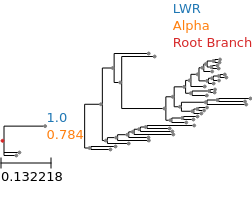
\includegraphics[width=.4\linewidth]{figs/early_stop_tests/es_test_cds12_no_outgroup.png}
%    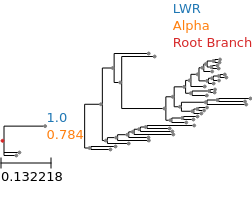
\includegraphics[width=.4\linewidth]{figs/early_stop_tests/es_test_cds12_no_outgroup_noes.png}
%    \caption{Effect of early stopping on results. Left is with early stopping,
%    Left is without. Dataset is AngiospermsCDS12}
%    \label{fig:es_angio}
%  \end{center}
%\end{figure}
\begin{figure}[H]
  \begin{center}
    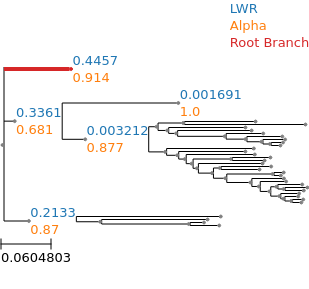
\includegraphics[width=.4\linewidth]{figs/early_stop_tests/es_test_mito_no_outgroup.png}
    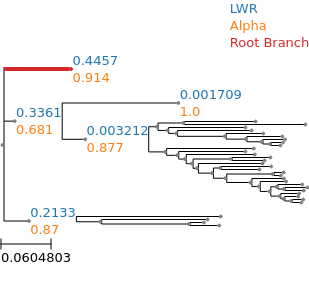
\includegraphics[width=.4\linewidth]{figs/early_stop_tests/es_test_mito_no_outgroup_noes.png}
    \caption{Effect of early stopping on results. Left is with early stopping,
    Left is without. Dataset is SpidersMitocondrial.}
    \label{fig:es_mito}
  \end{center}
\end{figure}

\section{Discussion}

\RootDiggertt{} is substantially faster than IQ-TREE, as is shown when comparing
figures \ref{fig:iq_time_results} and \ref{fig:rd_time_results}. Furthermore,
the accuracy of root placement of \RootDiggertt{} is nearly the same as IQ-TREE.

In Huelsenbeck \cite{huelsenbeck_inferring_2002}, it was shown that the prior
probability of a root placement on a sample tree did not have a strong signal.
When peforming our verficiation of \RootDiggertt{} using emperical data, we
found that this was often not the case. For example on the AngiospermsCDS12
dataset (see figure \ref{fig:angio-cds12-no-outgroup}), we found a clear signal
for the root placcment. Even in cases when the signal was not as strong, for
example SpidersMitocondrial (see figure \ref{fig:spiders-mito-no-outgroup}),
there is a much stronger signal for root placment than Huelsenbeck would suggest
we would get with this kind of analysis (which is to say, non-reversible
subsitution analysis). We suspect that this is due to Huelsenbeck performing the
analysis on a 4 taxon tree. By only using 4 taxa, the rate matrix is less
constrained by the data present, which leads to overfitting the rate matrix. 



\section{Conclusion}

We have shown that some datasets are particularly well suited to this form of
analysis, and that \RootDiggertt{} can be a simple alternative to similar forms
of root inference, such as molecular clock anaylsis or the use of an outgroup.

\bibliographystyle{acm}
\bibliography{main}

\end{document}
